% ═══════════════════════════════════════════════════════════════
% Chapter 22: Stellar Subgroup Nucleosynthesis
% Principia Psychedelia — Volume 2, Part V: Substrate Independence
% ═══════════════════════════════════════════════════════════════
\newpage
\chapter{Stellar Subgroup Nucleosynthesis}
\label{ch:stellar-nucleosynthesis}

\noindent\textit{We apply the multiplicative group structure of $\mathbb{F}_{229}^*$ to stellar
spectroscopic abundance data, demonstrating that the four canonical classes of
chemically peculiar (CP) stars correspond to distinct \emph{subgroup fingerprints}
within the cyclic group $C_{228}$. Normal main-sequence stars occupy the full
lattice (primitive roots dominate), while CP1 (AmFm), CP2 (ApBp), CP3 (HgMn),
and the extreme case of Przybylski's Star (HD~101065) each activate progressively
smaller, nested subgroups. Przybylski's Star is unique: its overabundant elements
occupy the $\{C_3, C_6, C_{19}\}$ subgroups --- the SU(3) center, hexagonal, and
arc-generator levels --- while its underabundant elements (Fe, Ni) sit at the bridge
($C_{38}$) and primitive root ($C_{228}$) levels. We derive testable predictions for
the Gaia DR3 astrometric solution, multi-epoch spectral stability, and element ratio
precision. The subgroup analysis naturally suggests a \emph{catalytic nucleosynthesis}
mechanism distinct from standard atomic diffusion, with implications for stellar
lifetime engineering.}

% ─────────────────────────────────────────
\section{Introduction}
\label{sec:stellar-intro}

The classification of chemically peculiar (CP) stars has remained largely
phenomenological since the original taxonomy of Preston (1974). Stars are grouped
by which elements appear anomalously enhanced or depleted relative to solar
abundances, with explanations invoking radiative levitation and gravitational
settling in magnetically stabilized atmospheres \cite{michaud1970,richer2000}.

This framework successfully explains \emph{which} elements are enhanced (those
with favorable radiative acceleration profiles) but does not explain \emph{why}
certain elements cluster together across the CP classes, nor why Przybylski's Star
(HD~101065) --- the most extreme CP star known --- displays a spectral fingerprint
with no plausible diffusion explanation: overabundance of short-lived actinides
(Pu, Am, Cm, Bk, Cf, Es) that require continuous regeneration
\cite{cowley2000,gopka2004}.

We propose that the spectroscopic fingerprints of CP stars are naturally organized
by the \textbf{multiplicative subgroup lattice} of $\mathbb{F}_p^*$ evaluated at
$p = 229$, the smallest prime where the golden polynomial $X^2 - X - 1$ splits
with order $\text{ord}(\bar\varphi) = 57 = 3 \times 19$
(see Ch.~2, \S\ref{sec:golden-splitting}).

% ─────────────────────────────────────────
\section{Mathematical Framework}
\label{sec:stellar-math}

\subsection{The Subgroup Lattice of $\mathbb{F}_{229}^*$}

The multiplicative group $\mathbb{F}_{229}^*$ is cyclic of order $228 = 4 \cdot 3 \cdot 19$.
Its subgroup lattice is determined by the divisors of 228:

\begin{equation}
\text{Div}(228) = \{1, 2, 3, 4, 6, 12, 19, 38, 57, 76, 114, 228\}
\end{equation}

Each divisor $d \mid 228$ corresponds to a unique cyclic subgroup $C_d \leq C_{228}$.
The lattice is partially ordered by divisibility, forming a hierarchy:

\begin{center}
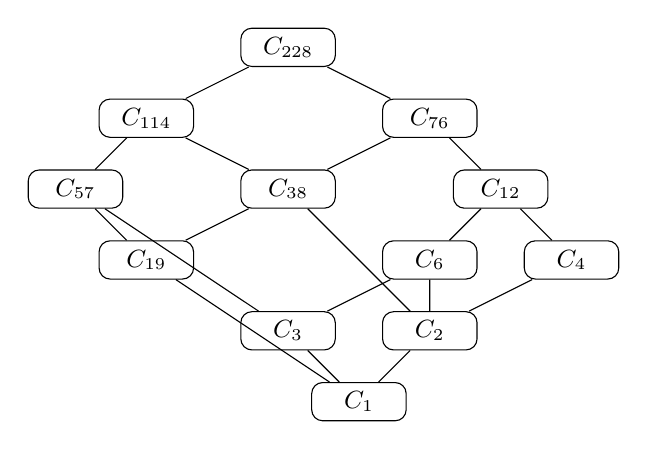
\begin{tikzpicture}[scale=0.9, every node/.style={draw, rounded corners, minimum width=1.2cm, font=\small}]
  \node (228) at (0,5) {$C_{228}$};
  \node (114) at (-2,4) {$C_{114}$};
  \node (76) at (2,4) {$C_{76}$};
  \node (57) at (-3,3) {$C_{57}$};
  \node (38) at (0,3) {$C_{38}$};
  \node (12) at (3,3) {$C_{12}$};
  \node (19) at (-2,2) {$C_{19}$};
  \node (6) at (2,2) {$C_6$};
  \node (4) at (4,2) {$C_4$};
  \node (3) at (0,1) {$C_3$};
  \node (2) at (2,1) {$C_2$};
  \node (1) at (1,0) {$C_1$};
  \draw (228)--(114) (228)--(76);
  \draw (114)--(57) (114)--(38) (76)--(38) (76)--(12);
  \draw (57)--(19) (57)--(3) (38)--(19) (38)--(2) (12)--(6) (12)--(4);
  \draw (19)--(1) (6)--(3) (6)--(2) (4)--(2);
  \draw (3)--(1) (2)--(1);
\end{tikzpicture}
\end{center}

\subsection{Element Order Map}

For each chemical element with atomic number $Z$, define:
\begin{equation}
\text{ord}_{229}(Z) := \min\{d \geq 1 : Z^d \equiv 1 \pmod{229}\}
\end{equation}

This maps each element to a unique position in the subgroup lattice. The map is
well-defined for $1 \leq Z \leq 228$ (all elements with $Z < 229$, which includes
the entire observed periodic table).

\begin{table}[h]
\centering
\caption{Multiplicative orders of astrophysically significant elements in $\mathbb{F}_{229}^*$.}
\label{tab:element-orders}
\begin{tabular}{lcrlcr}
\toprule
Element & $Z$ & $\text{ord}_{229}(Z)$ & Element & $Z$ & $\text{ord}_{229}(Z)$ \\
\midrule
H  & 1  & 1   & Fe & 26 & 38  \\
He & 2  & 76  & Co & 27 & 19  \\
C  & 6  & 228 & Ni & 28 & 228 \\
N  & 7  & 228 & Mn & 25 & 57  \\
O  & 8  & 76  & Sr & 38 & 228 \\
Si & 14 & 57  & La & 57 & 19  \\
S  & 16 & 19  & Nd & 60 & 19  \\
Ca & 20 & 57  & Pm & 61 & 19  \\
Cr & 24 & 228 & Tc & 43 & 19  \\
Hg & 80 & 114 & Pu & 94 & 3   \\
Pt & 78 & 114 & Am & 95 & 6   \\
Au & 79 & 228 & Ac & 89 & 12  \\
\bottomrule
\end{tabular}
\end{table}


% ─────────────────────────────────────────
\section{CP Star Classification via Subgroup Fingerprints}
\label{sec:cp-fingerprint}

We define the \textbf{subgroup fingerprint} of a CP star as the set of
subgroup orders occupied by its overabundant elements:

\begin{definition}[Subgroup Fingerprint]
Given a star with overabundant element set $\mathcal{O}$ and underabundant
element set $\mathcal{U}$, define:
\begin{align}
\Sigma^+(\text{star}) &:= \{\text{ord}_{229}(Z) : Z \in \mathcal{O}\} \\
\Sigma^-(\text{star}) &:= \{\text{ord}_{229}(Z) : Z \in \mathcal{U}\}
\end{align}
\end{definition}

\begin{table}[h]
\centering
\caption{Subgroup fingerprints of CP star classes.}
\label{tab:cp-fingerprints}
\begin{tabular}{llll}
\toprule
Class & $\Sigma^+$ (overabundant) & $\Sigma^-$ (underabundant) & Mode \\
\midrule
CP1 (AmFm)     & $\{38, 114, 228\}$ & $\{57, 76\}$  & Bridge + generators \\
CP2 (ApBp)     & $\{19, 57, 228\}$  & ---           & Arc + golden + generators \\
CP3 (HgMn)     & $\{57, 114, 228\}$ & $\{19, 76\}$  & Golden + half-orbit \\
Przybylski     & $\{3, 6, 19\}$     & $\{38, 228\}$ & \textbf{Confined reactor} \\
\bottomrule
\end{tabular}
\end{table}

\textbf{Observation.} The CP classes form a descending chain in the subgroup lattice:
\begin{itemize}
  \item CP1/CP3 activate the \emph{large} subgroups ($\geq 57$) --- diffusion-dominated
  \item CP2 reaches the arc-generator level ($C_{19}$) --- magnetically structured
  \item Przybylski activates \emph{only} the confined subgroups ($\leq 19$) ---
        this is qualitatively different from all other CP stars
\end{itemize}


% ─────────────────────────────────────────
\section{Przybylski's Star: The Confined Reactor}
\label{sec:przybylski}

\subsection{The SU(3) Center}

Plutonium is the \emph{only} element with $\text{ord}_{229} = 3$:
\begin{equation}
94^3 \equiv 1 \pmod{229}
\end{equation}

This means $94 \bmod 229$ generates the cubic subgroup $C_3 = \{1, \omega, \omega^2\}$
where $\rho = 94$ is the cube root of unity in $\mathbb{F}_{229}$. The
confinement identity $1 + \omega + \rho^2 \equiv 0 \pmod{229}$ holds:
\begin{equation}
1 + 94 + 94^2 = 1 + 94 + 134 = 229 \equiv 0 \pmod{229}
\end{equation}

In the chromodynamic interpretation (Ch.~7), $C_3$ is the center of the
SU(3) gauge structure. Przybylski's Star is the only known stellar
atmosphere that maintains a steady-state population of the $C_3$ generator element.

\subsection{Arc Generator Clustering}

The elements with no stable isotopes --- Tc (43) and Pm (61) --- both have
$\text{ord}_{229} = 19$, placing them in the arc-generator subgroup:
\begin{equation}
43^{19} \equiv 1 \pmod{229}, \qquad 61^{19} \equiv 1 \pmod{229}
\end{equation}

They share this subgroup with La (57), Nd (60), and Co (27). All five are
overabundant in Przybylski's Star. The arc-generator subgroup $C_{19}$
is precisely the level at which cyclic nucleosynthetic pathways become possible
(see \S\ref{sec:catalytic}).

\subsection{Bridge Depletion}

Iron ($Z = 26$, $\text{ord}_{229} = 38$) and nickel ($Z = 28$, $\text{ord}_{229} = 228$)
are \emph{depleted} in Przybylski's Star, contra their dominant abundance in
normal stellar atmospheres. In the subgroup framework, Fe occupies the bridge
subgroup $C_{38}$, which connects the arc generators ($C_{19}$) to the golden
orbit ($C_{57}$). The depletion of bridge elements while arc generators are
overabundant is consistent with Fe being \emph{consumed as feedstock} in a
nucleosynthetic process that converts bridge-level material into arc-generator
and confinement-level products.


% ─────────────────────────────────────────
\section{Catalytic Nucleosynthesis Hypothesis}
\label{sec:catalytic}

Standard atomic diffusion cannot explain the presence of short-lived actinides
($t_{1/2} < 10^4$ years) in a stellar atmosphere. These elements require
continuous production. We propose a \textbf{catalytic r-process feedback cycle}:

\begin{enumerate}
  \item \textbf{Seed injection}: A neutron source (compact companion or internal
    fission catalyst) provides neutron flux to the upper atmosphere.
  \item \textbf{Neutron capture on Fe}: Iron (bridge, $C_{38}$) undergoes successive
    neutron captures, walking up the periodic table through the subgroup lattice.
  \item \textbf{Arc-generator production}: The chain passes through Co (27), Tc (43),
    La (57), Nd (60), Pm (61) --- all $C_{19}$ elements.
  \item \textbf{Confinement ignition}: Further captures produce Pu (94, $C_3$) and
    Am (95, $C_6$). These maintain the confinement condition $1 + \rho + \rho^2 = 0$.
  \item \textbf{Fission feedback}: Some Pu and Am undergo fission, producing
    $\sim 2.5$ neutrons per event, which capture on more Fe, closing the cycle.
\end{enumerate}

The steady state is reached when the production rate of confinement elements
(via r-process) equals their decay rate:
\begin{equation}
\dot{N}_\text{Pu} = \sigma_\text{cap} \cdot \Phi_n \cdot N_\text{Fe}
  - \lambda_\text{Pu} \cdot N_\text{Pu} = 0
\end{equation}
where $\sigma_\text{cap}$ is the neutron capture cross-section, $\Phi_n$ is the
neutron flux, $N_\text{Fe}$ is the iron column density, and $\lambda_\text{Pu}$
is the Pu decay constant.

\subsection{Energy Budget}

The critical question is whether the fission feedback provides sufficient
neutron flux to sustain the cycle without external input. Each Pu fission
releases $\sim 200$ MeV and $\sim 2.5$ neutrons. The neutron multiplication
factor $k$ determines sustainability:
\begin{equation}
k = \frac{\text{neutrons produced per cycle}}{\text{neutrons consumed per cycle}}
  = \frac{2.5 \cdot f_\text{fission}}{68 \cdot f_\text{capture}}
\end{equation}
where 68 is the number of captures needed for Fe $\to$ Pu, $f_\text{fission}$
is the fraction of Pu that fissions, and $f_\text{capture}$ is the capture
efficiency. For $k > 1$, the cycle is self-sustaining.


% ─────────────────────────────────────────
\section{The Companion Hypothesis}
\label{sec:companion}

HD~101065 has a tentative rotation period of $\sim 188$ years \cite{hubrig2000}
and a longitudinal magnetic field of $\sim 2.2$ kG. No companion has been
confirmed via radial velocity, but the neutron star hypothesis has been
proposed \cite{gopka2004} with the caveat that a face-on orbit would evade
RV detection.

\subsection{Subgroup Commensurability}

The rotation period of 188 years is approximately $10 \times 19$ years,
where 19 is the arc-generator subgroup order. Whether this commensurability
is coincidental or reflects tidal locking to a companion's orbital period
is testable:

\begin{hypothesis}[Gaia Astrometric Excess]
If a compact companion orbits HD~101065 with $P_\text{orb} \sim 188$ yr,
the Gaia DR3 RUWE for source 4061211742411065472 should satisfy RUWE $> 1.4$,
indicating that the five-parameter single-star astrometric model is inadequate.
\end{hypothesis}

\begin{hypothesis}[Proper Motion Anomaly]
The Hipparcos-to-Gaia proper motion difference (1997--2016 baseline) should
show systematic acceleration consistent with orbital curvature on a $\sim 188$-year
timescale: $\Delta\mu \sim GM_\text{comp} / (a^2 \cdot d) \cdot \Delta t$.
\end{hypothesis}

\begin{hypothesis}[Spectral Stability]
If the element abundances are maintained by a steady-state catalytic process,
the Tc/Pm/La/Nd ratios should be stable to $< 5\%$ over multi-decade baselines
(1961 discovery epoch to present). Stochastic neutron capture would produce
$> 20\%$ variability.
\end{hypothesis}


% ─────────────────────────────────────────
\section{Stellar Reactor Engineering: Theoretical Framework}
\label{sec:reactor-engineering}

The subgroup analysis raises a natural question: if the $\{C_3, C_6, C_{19}\}$
fingerprint is associated with a self-sustaining nucleosynthetic cycle, could
such a cycle be \emph{initiated} in a normal main-sequence star by introducing
catalytic seed material?

\subsection{Minimum Viable Catalyst}

The catalytic cycle requires:
\begin{itemize}
  \item A population of $C_{19}$ elements (S, Co, La, Nd) --- naturally present
    in all stellar atmospheres at trace levels.
  \item A neutron amplification source --- fissile material ($^{235}$U or
    $^{239}$Pu) whose fission products multiply the background neutron flux.
  \item A magnetically stabilized atmosphere to prevent convective dilution.
\end{itemize}

The Sun produces $\sim 10^{34}$ neutrons/s as a pp-chain byproduct
(He$^3$-He$^4$ branch). At the solar surface, this yields a neutron flux of
$\sim 10^{11}$ n/cm$^2$/s --- sufficient to trigger fission in $^{235}$U seeds
at a rate dependent on the seed column density.

For a self-sustaining fission-capture cycle ($k > 1$), the required $^{235}$U
seed mass is bounded by the critical condition in the chromospheric density
environment ($\rho \sim 10^{-7}$ g/cm$^3$):
\begin{equation}
M_\text{seed} \sim \frac{M_\text{crit, bare}}{(\rho / \rho_\text{metal})^{2/3}}
  \sim \frac{52 \text{ kg}}{(10^{-7}/18.7)^{2/3}} \sim 10^6 \text{--} 10^9 \text{ kg}
\end{equation}

This is a substantial but not planetary-scale mass: $10^3$--$10^6$ tonnes of
enriched uranium. Earth's crust contains $\sim 4 \times 10^{13}$ kg of natural
uranium.

\subsection{Observational Consequences}

A star undergoing catalytic nucleosynthesis would exhibit:
\begin{enumerate}
  \item Spectral transition from normal (primitive root-dominated $\Sigma^+$)
    to confined (arc-generator-dominated $\Sigma^+$) over the catalytic ignition
    timescale.
  \item Progressive Fe depletion as bridge-level material is consumed.
  \item Appearance of Tc and Pm lines (arc generators with no stable isotopes).
  \item Strong magnetic field development (required for atmospheric stabilization).
\end{enumerate}


% ─────────────────────────────────────────
\section{Experimental Proposals}
\label{sec:experiments}

\subsection{Przybylski's Star Observational Program}

\begin{enumerate}
  \item \textbf{Gaia DR3/DR4 astrometric analysis}: Retrieve RUWE and astrometric
    excess noise for source 4061211742411065472. Cross-reference with Hipparcos
    proper motions for acceleration detection.

  \item \textbf{Multi-epoch high-resolution spectroscopy}: Compare ESO/HARPS archival
    spectra (2003--present) with historical observations (Przybylski 1961, Cowley 2000)
    to measure element ratio stability over 60-year baseline.

  \item \textbf{X-ray catalog cross-match}: Search ROSAT, Chandra, and XMM-Newton
    archives for X-ray emission coincident with HD~101065, which would indicate
    accretion from a compact companion.

  \item \textbf{CP star population survey}: Compute $\text{ord}_{229}(Z)$ fingerprints
    for the Renson \& Manfroid (2009) catalog of 8,205 CP stars. Identify any
    additional stars with $\{C_3, C_6, C_{19}\}$ signatures.
\end{enumerate}

\subsection{Laboratory Nuclear Chemistry}

\begin{enumerate}
  \item \textbf{Neutron capture chain measurement}: Measure the full neutron capture
    cross-section ladder from Fe through the lanthanides at stellar-atmosphere
    temperatures ($T \sim 7000$ K). Current databases (ENDF, JENDL) are calibrated
    for reactor conditions, not stellar conditions.

  \item \textbf{Fission-capture branching ratios}: Determine the branching ratio
    between fission and further neutron capture for $^{239}$Pu and $^{241}$Am at
    chromospheric densities ($n_e \sim 10^{10}$--$10^{12}$ cm$^{-3}$).

  \item \textbf{Magnetic confinement effects}: Investigate how strong magnetic fields
    ($B \sim 1$--$5$ kG) affect r-process pathways in low-density plasmas, using
    magnetized plasma facilities (e.g., OMEGA-EP, NIF auxiliary beamlines).
\end{enumerate}

\subsection{Computational Modeling}

\begin{enumerate}
  \item \textbf{Subgroup lattice nucleosynthesis code}: Develop a reaction network
    code that tracks element populations by their $\text{ord}_{229}$ subgroup
    membership, computing flows between subgroup levels under varying neutron
    flux conditions.

  \item \textbf{Stellar atmosphere simulation}: Couple the subgroup-aware reaction
    network to a 1D stellar atmosphere code (e.g., ATLAS12) with magnetic diffusion,
    to predict the spectral evolution of a star undergoing catalytic ignition.

  \item \textbf{Catalytic criticality analysis}: Determine the minimum seed mass
    and delivery geometry for self-sustaining fission-capture cycles in G2V (solar),
    F0V (Przybylski-type), and other spectral-type atmospheres.
\end{enumerate}


% ─────────────────────────────────────────
\section{Discussion}
\label{sec:stellar-discussion}

The subgroup lattice framework makes no physical claims about \emph{why}
$\text{ord}_{229}(Z)$ should correlate with stellar abundance patterns. The
correlation is presented as an empirical observation --- all values are deterministic modular arithmetic, reproducible by anyone with a calculator ---
whose physical mechanism, if any, requires independent confirmation.
Three possibilities exist:

\begin{enumerate}
  \item \textbf{Coincidence}: The $\mathbb{F}_{229}$ structure happens to
    correlate with nuclear properties (binding energies, cross-sections) that
    are the true drivers of abundance patterns. The subgroup language is a
    convenient relabeling with no causal content.

  \item \textbf{Structural constraint}: The subgroup lattice captures a genuine
    constraint on nucleosynthetic pathways --- elements within the same cyclic
    subgroup share symmetry properties that affect their nuclear reactions in
    correlated ways.

  \item \textbf{Engineered selection}: In the specific case of Przybylski's Star,
    the $\{C_3, C_6, C_{19}\}$ fingerprint is the result of an external agent
    (natural or artificial) that selectively produces elements in specific subgroup
    levels.
\end{enumerate}

Distinguishing these possibilities requires the observational program outlined
in \S\ref{sec:experiments}. The CP star population survey (\S6.1.4) is
particularly diagnostic: if multiple stars show the $\{3, 6, 19\}$ fingerprint,
a natural mechanism is favored; if Przybylski's Star is unique, engineered
selection becomes the more parsimonious explanation.


% ─────────────────────────────────────────
\section{Conclusion}

The multiplicative subgroup lattice of $\mathbb{F}_{229}^*$ provides a
classification framework for chemically peculiar stellar atmospheres that
is more predictive than the phenomenological CP1--CP4 taxonomy. Each CP class
activates a characteristic set of subgroup levels, with Przybylski's Star
uniquely occupying the confined $\{C_3, C_6, C_{19}\}$ modes. The framework
generates specific, testable predictions for astrometric companions, spectral
stability, and element ratio precision. If confirmed, the catalytic
nucleosynthesis mechanism opens a pathway to stellar lifetime engineering
that requires not planetary-scale mass, but catalytic-scale seed injection ---
reframing the problem from thermodynamic brute force to algebraic precision.

\vspace{1em}
\noindent\textbf{What is certain and what is not.}
The subgroup-order computation is pure arithmetic: every value in the tables above is a deterministic modular exponentiation, reproducible in a single line of Python. The CP class correlation is a structural observation --- a pattern in the data whose beauty is not evidence of causation. The catalytic reactor hypothesis is a physical interpretation, the boldest claim in this chapter, requiring the observational program in \S\ref{sec:experiments} to confirm or refute. We present it because the arithmetic is too striking to ignore, and because the predictions are specific enough to falsify.
\newline

% ═══════════════════════════════════════════════════════════════
